% Appendix B. GNURadio Companion
%==========================================================================

\chapter{GNURadio Companion}
\label{AppB}

\emph{GNURadio} incluye una aplicaci\'on que facilita el desarrollo de grafos y aplicaciones
sencillas de manera gr\'afica, muy similar al software de Simulink de Mathworks. La aplicaci\'on
genera c\'odigo en \emph{Python} apartir del diagrama de bloques. Es posible manipular y
extender el c\'odigo generado si se desea utilizar alguna funci\'on que no est\'e incluida en
\emph{GNURadio Companion}\cite{grc} (GRC por sus siglas en \emph{Ingl\'es}). Las capacidades de la
aplicaci\'on son:

\begin{itemize}
  \item Viene incluido con el c\'odigo fuente de \emph{GNURadio}. Si se instalan todas las dependencias
  entonces GRC se instalar\'a junto con \emph{GNURadio}.
  \item Puede generar c\'odigo en \emph{Python} para aplicaciones que utilizan bloques gr\'aficos con la
  librer\'ia WxWidgets, aplicaciones que no utilizan ning\'un control gr\'afico y bloques jer\'arquicos.
  \item Se pueden definir bloques que actuan como variables o constantes. Otros bloques pueden hacer
  referencia a ellas e incluir su valor en alg\'un par\'ametro. Tambien es posible usar bloques
  variables que definen un control gr\'afico como barras deslizadoras, botones, etc.
  \item Cada bloque est\'a definido por un archivo XML que contiene todas sus caracteristicas (n\'umero
  de puertos, tipo de datos con los que trabaja, par\'ametros de entrada, etc.). Es posible crear un
  archivo XML para incluir alg\'un bloque creado por el usuario.
  \item Los bloques pueden ser deshabilitados dentro de la gr\'afica sin tener que borrarlos de la
  aplicaci\'on. Estos bloques son ignorados por el generador de c\'odigo, permitiendo as\'i una manera
  m\'as r\'apida de realizar cambios en la gr\'afica. Tambien se pueden cortar, copiar y pegar bloques.
\end{itemize}

Para instalar GRC se debe tener las siguientes dependencias intaladas antes de iniciar la
compilaci\'on:

\begin{itemize}
  \item Python 2.5 o mayor (\url{http://www.python.org/download/})
  \item Python-LXML 2.0 o  mayor (\url{http://codespeak.net/lxml/installation.html})
  \item Cheetah Template Engine 2.0 o mayor (\url{http://www.cheetahtemplate.org/download.html})
  \item Python-GTK 2.10 o mayor (\url{http://www.pygtk.org/downloads.html})
\end{itemize}

Si estas dependencias se instalan antes de iniciar con la compilaci\'on de \gnuradio entonces GRC se
instalar\'a autom\'aticamente.

Para iniciar la aplicaci\'on se necesita abrir una ventana de consola y escribir el comando
\verb|gnuradio-companion|. Inmediatamente aparecer\'a la ventana que se muestra en la figura
\ref{fig:grc}.

\begin{figure}[tp]
  \centering
  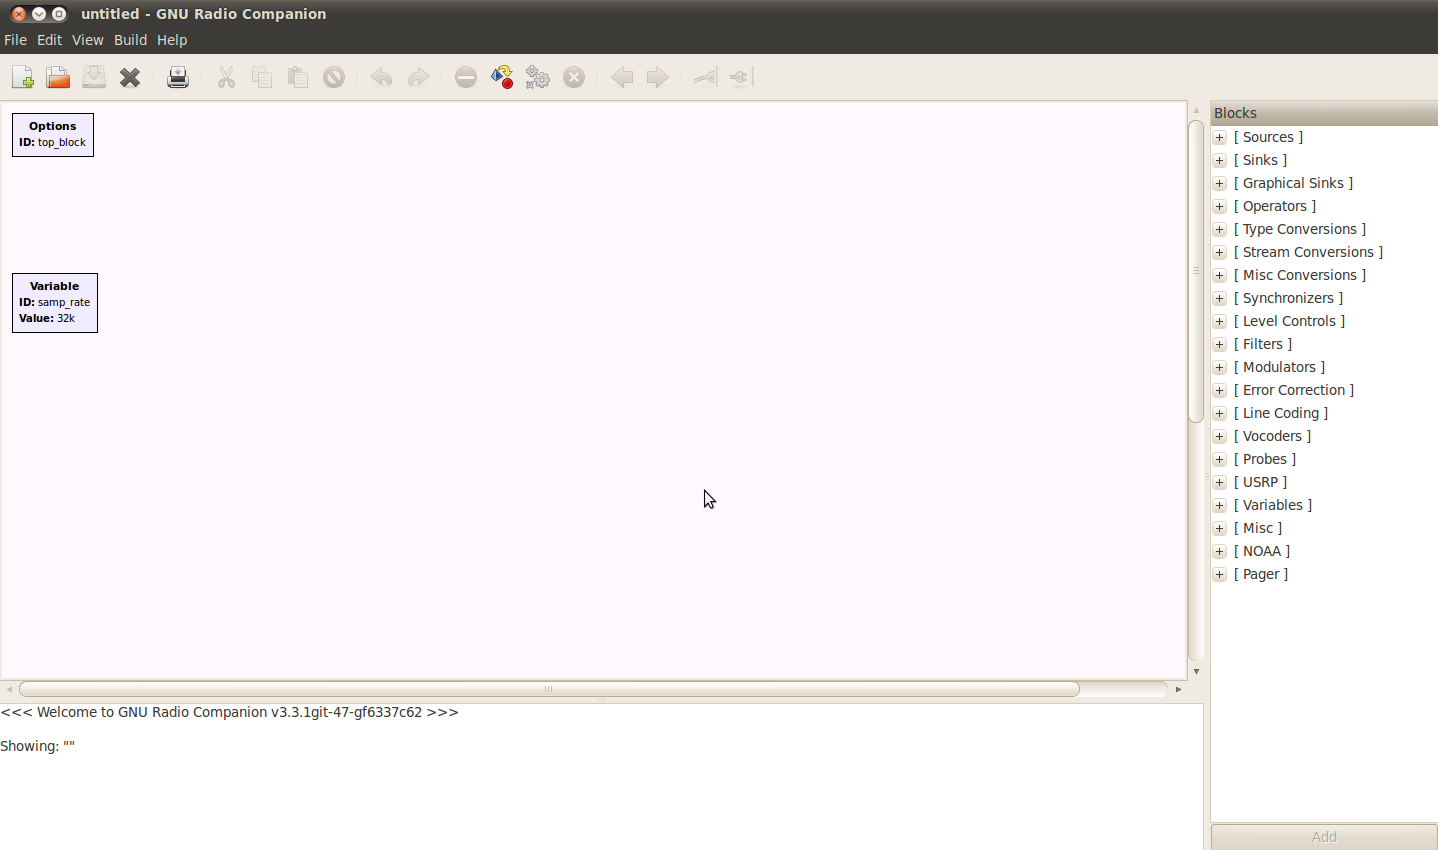
\includegraphics[width=5.5in]{figs/grc1}
  \vspace{0.1in}
  \caption{Pantalla principal de \emph{GNURadio Companion}}
  \label{fig:grc}
\end{figure}

El \'area de trabajo inicia con dos bloques por default, uno que define las opciones generales del
grafo y un bloque que define una variable llamada \verb|sample_time|. Esta variable se puede
modificar o borrar seg\'un las necesidades del usuario. Del lado derecho se encuentra la lista de las
categor\'ias de bloques que soporta GRC. Cada categor\'ia se puede expandir para revelar los
diferentes bloques que contiene. Para colocar bloques en el \'area de trabajo es necesario
seleccionar el de inter\'es y arrastrarlo con el mouse a la area de trabajo. De ah\'i se puede seguir
arrastrando para colocarlo en el \'area que se desee. 

Las propiedades de los bloques se pueden obtener haciendo doble click sobre el bloque como se
muestra en la figura \ref{fig:blockprop}.

\begin{figure}[tp]
  \centering
  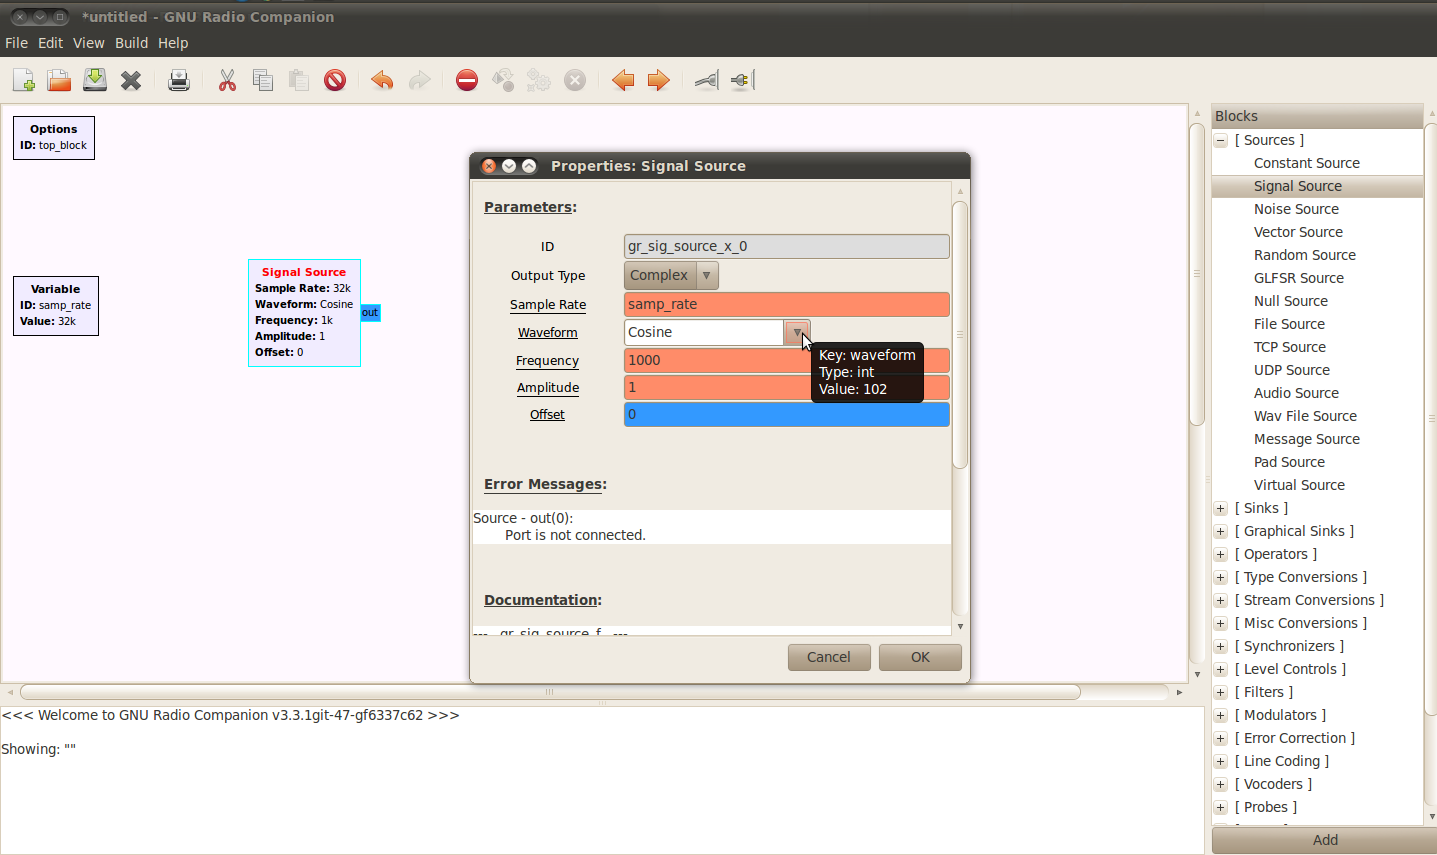
\includegraphics[width=5.5in]{figs/grc3}
  \vspace{0.1in}
  \caption{Pantalla de propiedades del bloque signal\_source}
  \label{fig:blockprop}
\end{figure}

Todos los bloques comparten un par\'ametro en com\'un y es el ID. Este par\'ametro indentifica al bloque
para que otros puedan hacer referencia a \'el. Se puede aceptar el nombre por defecto que GRC sugiere o
bien se puede especificar otro. Los otros par\'ametros son espec\'ificos del bloque con el que se est\'a
trabajando. El bloque \verb|signal_source| de la figura \ref{fig:blockprop} es un generador de
se\~nales que puede generar varios tipos de formas de onda como senoidales, cuadradas, dientes de
sierra, etc. Los par\'ametros se describen como sigue:

\begin{description}
\item[Output Type] Especifica el tipo de datos que utiliza para generar la forma de onda: Real o Complejo.
\item[Sample Rate] La tasa de muestreo con la que se generar\'a la se\~nal. Aqu\'i se muestra haciendo
referencia al bloque que declara la variable \verb|sample_rate|. Esta variable tiene un valor de
32k.
\item[Waveform] Aqu\'i se define el tipo de se\~nal que se quiere generar.
\item[Frequency] Este p\'arametro especifica la frecuencia de la se\~nal.
\item[Amplitude] Este p\'arametro especifica la amplitud de la se\~nal.
\item[Offset] Especifica un retraso de la se\~nal generada.
\end{description}

En la figura \ref{fig:grcex} se muestra un ejemplo completo de un grafo que suma dos se\~nales de
diferentes frecuencias y muestra el resultado en un osciloscopio.

\begin{figure}[tp]
  \centering
  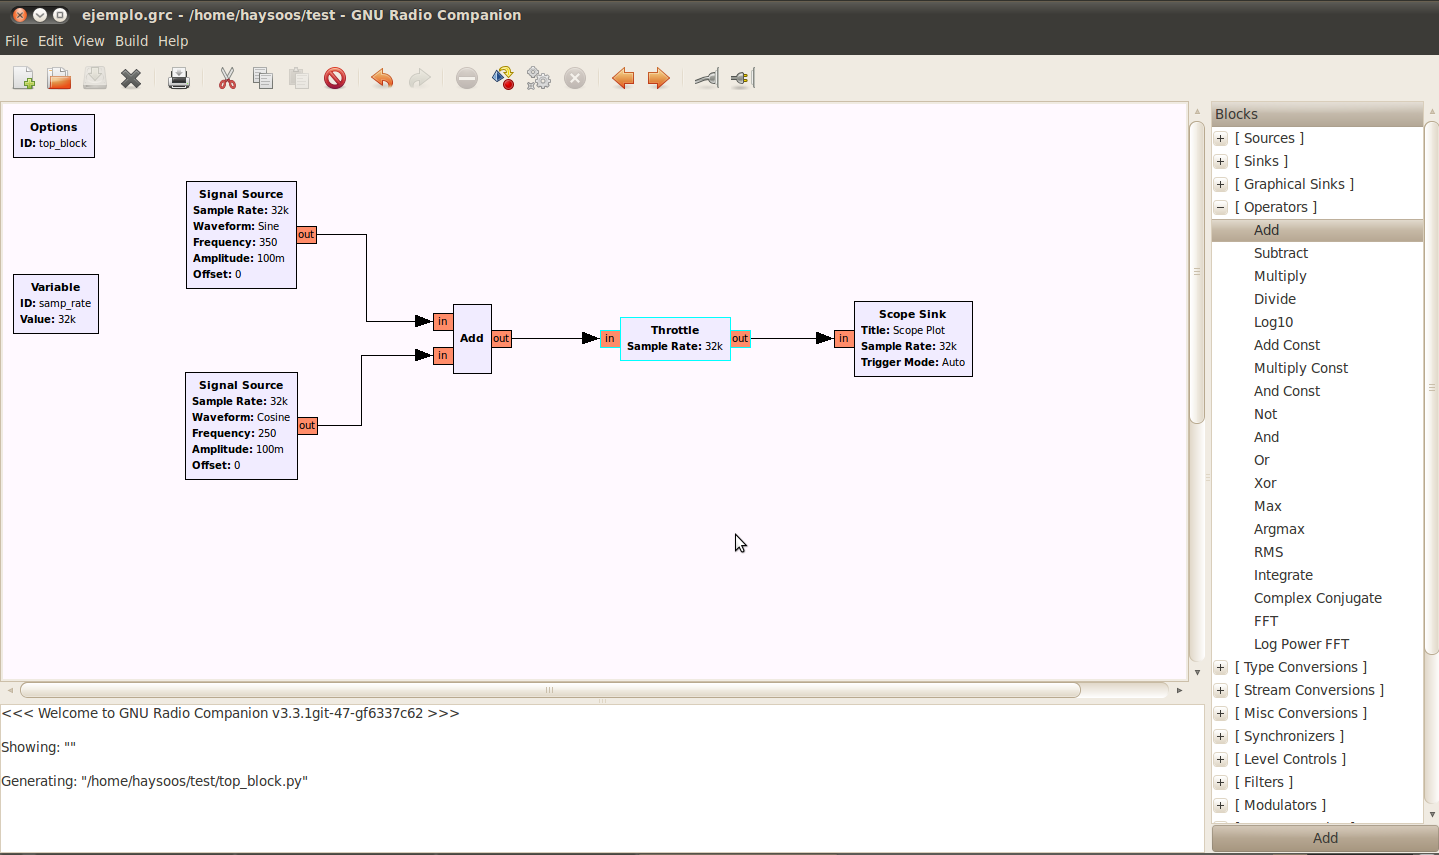
\includegraphics[width=5.5in]{figs/grc6}
  \vspace{0.1in}
  \caption{Ejemplo de un grafo desarrollado en GRC}
  \label{fig:grcex}
\end{figure}

El ejemplo muestra un requerimiento importante de los grafos que no utilizan fuentes o sinks de
hardware como el USRP o la tarjeta de sonido. Los bloques que hacen referencia a alg\'un hardware
limitan autom\'aticamente la velocidad de ejecuci\'on del grafo a la velocidad de muestreo del
hardware. Como el ejemplo de la figura \ref{fig:grcex} no contiene este tipo de bloques es
necesario incluir el bloque \verb|Throttle| para limitar la velocidad de ejecuci\'on, de lo
contrario el grafo se ejecutar\'a a la velocidad m\'axima del CPU y esto causara que la PC no
responda correctamente. Para este ejemplo el bloque hace referencia a la variable \verb|sample_rate|
declarada y con esto limita la velocidad de ejecuci\'on a la tasa de muestreo que se est\'a utilizando.

El bloque \verb|Scope Sink| es uno de los diversos visualizadores gr\'aficos que permiten observar las
se\~nales en diversos puntos del grafo. Este bloque actua como un osciloscopio con opciones de
disparo y modo XY. Otros bloques con los que cuenta GRC para visualizar se\~nales son: analizador de
espectros, espectrograma en 2D, histograma y diagrama de constelaci\'on.

Si existe un error en alguna de las conexiones, ya sea porque los tipos de datos son incompatibles
entre bloques, algunas de las opciones no est\'an correctamente configuradas o falta alg\'un puerto
por conectar, estos ser\'an enfatizados de color rojo. Es necesario realizar las correcciones que se
piden antes de generar el c\'odigo y poder ejecutar el grafo.

Para ejecutar el grafo es necesario hacer click en el bot\'on de generar c\'odigo o en el de ejecutar
grafo. Si no se ha grabado el trabajo GRC pedir\'a que se grabe antes de la ejecuci\'on como se
muestra en la figura \ref{fig:savegrc}. Una vez realizado esto, GRC genera un archivo con c\'odigo
\emph{Python} y este es el que se ejecuta. La figura \ref{fig:rungrc} muestra el grafo de la suma de las
dos se\~nales ejecutandose y mostrando los resultados en un osciloscopio.

\begin{figure}[htp]
  \centering
  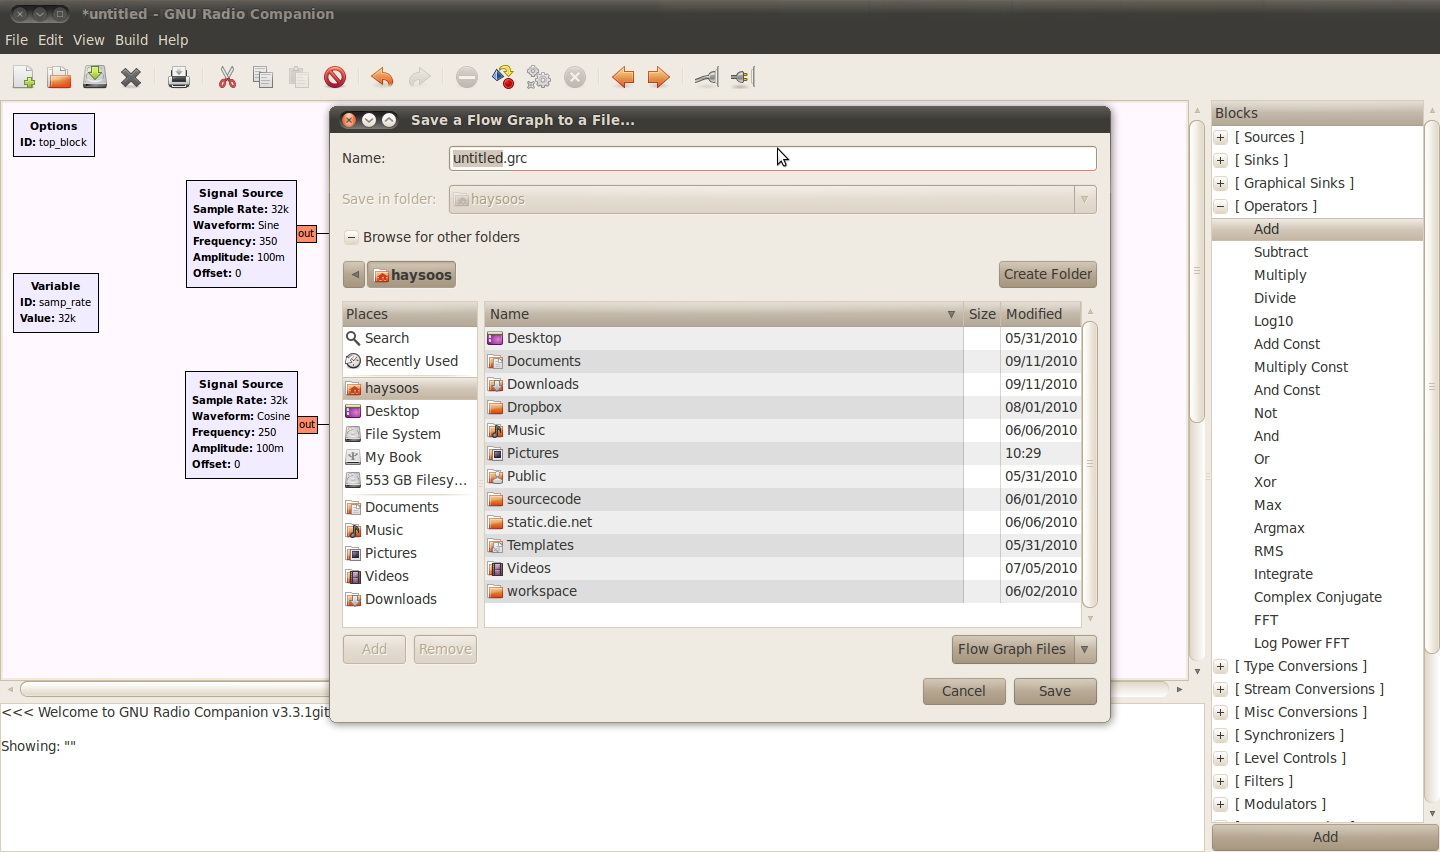
\includegraphics[width=5.5in]{figs/grc5}
  \vspace{0.1in}
  \caption{Pantalla para guardar el trabajo en GRC}
  \label{fig:savegrc}
\end{figure}

\begin{figure}[htp]
  \centering
  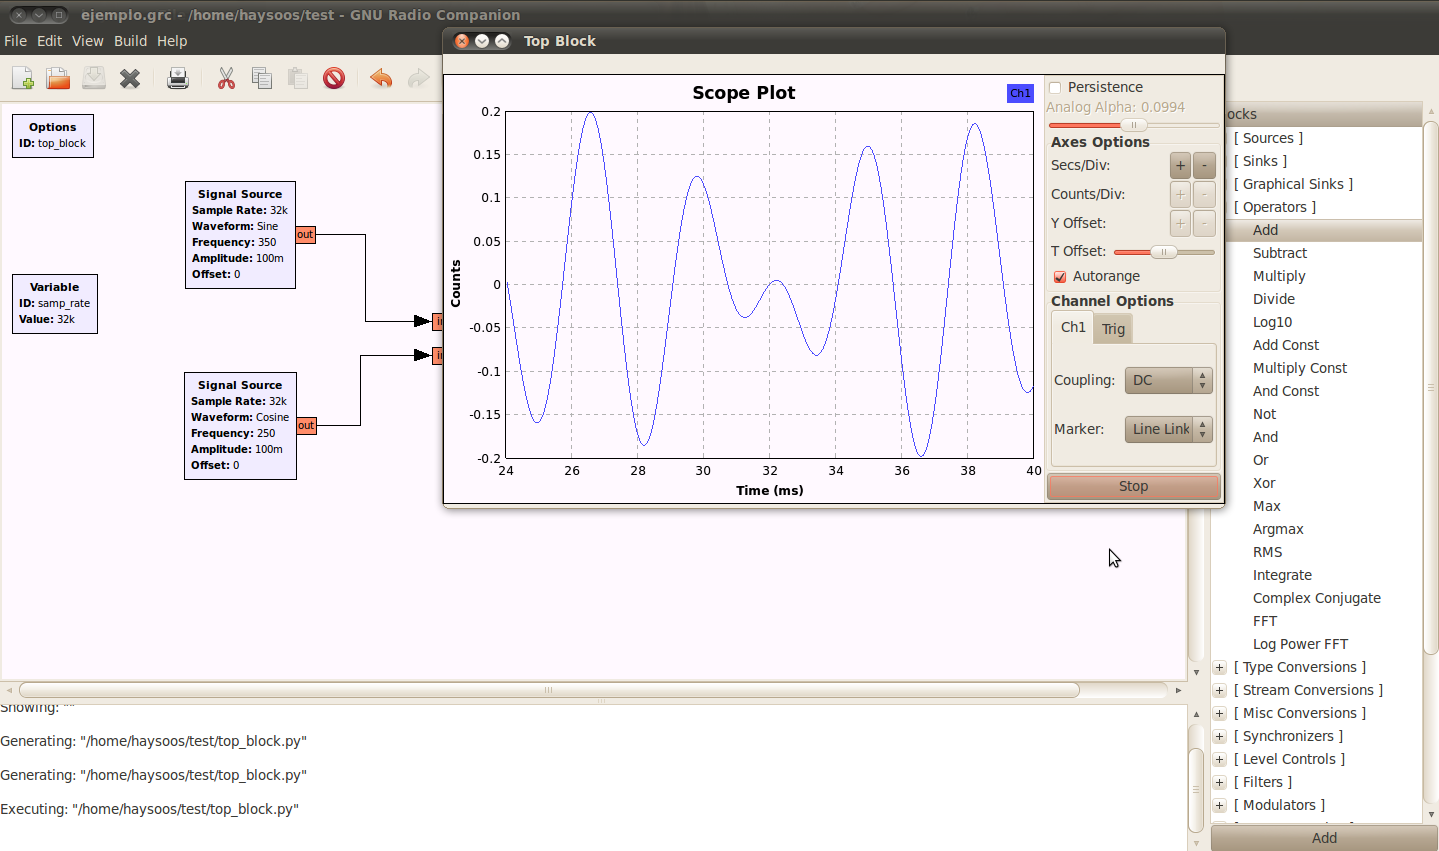
\includegraphics[width=5.5in]{figs/grc7}
  \vspace{0.1in}
  \caption{Ejemplo de un grafo en ejecuci\'on}
  \label{fig:rungrc}
\end{figure}

Conforme se vallan anexando bloques visualizadores, estos se van agrupando en la misma pantalla de
forma vertical. Esto permite visualizar los resultados de una manera m\'as eficiente sin tener que
estar cambiando entre diferentes ventanas. Agregando el bloque FFT al ejemplo obtenemos la pantalla
que se muestra en la figura \ref{fig:fftgrc}.

\begin{figure}[htp]
  \centering
  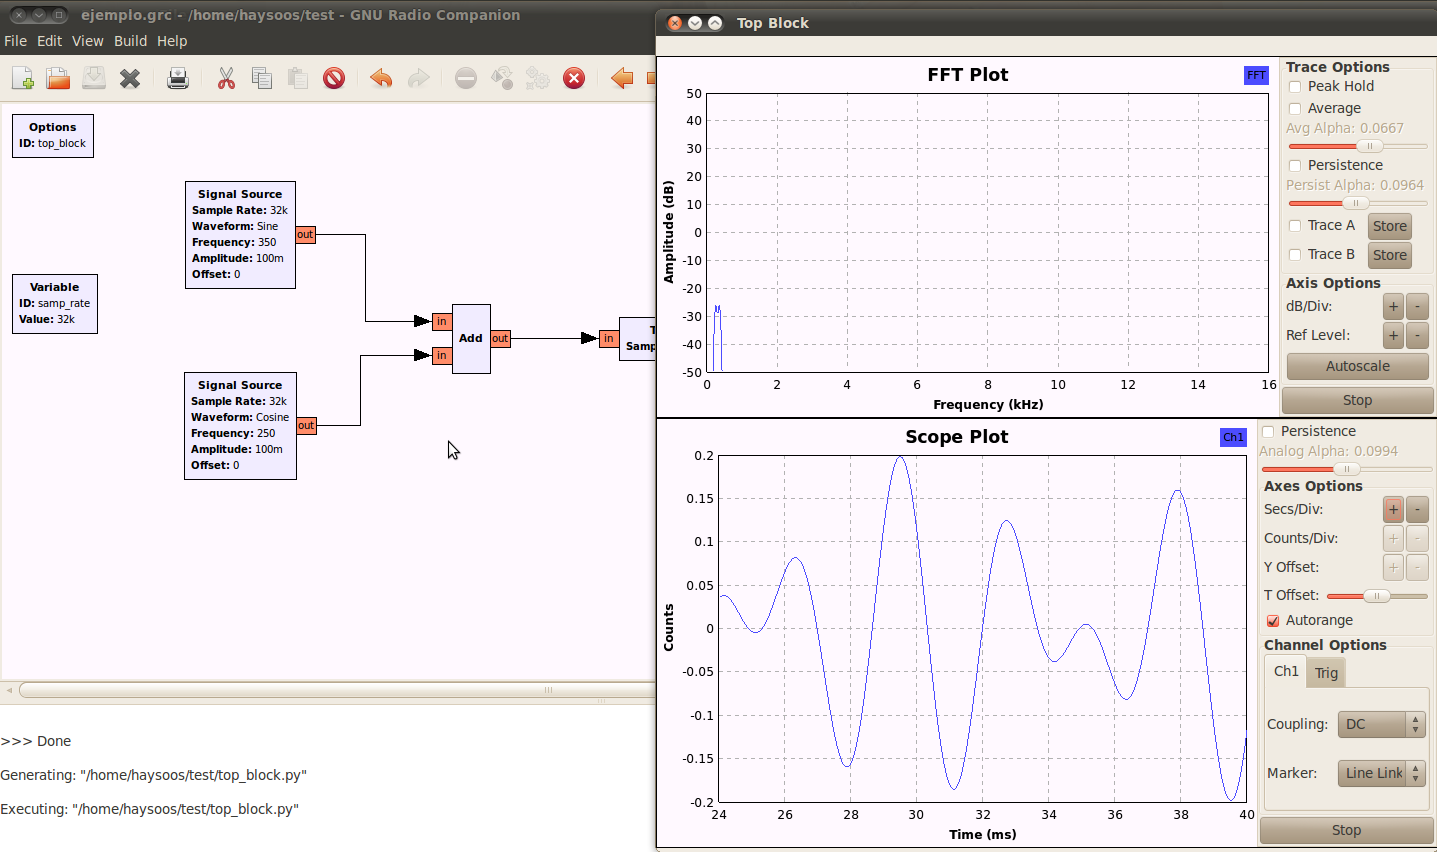
\includegraphics[width=5.5in]{figs/grc8}
  \vspace{0.1in}
  \caption{Bloque FFT en conjunto con el osciloscopio en GRC}
  \label{fig:fftgrc}
\end{figure}

Como se mencion\'o al inicio de este ap\'endice, una de las habilidades de GRC es poder especificar
bloques que implementan alg\'un tipo de control gr\'afico como barras deslizadoras. Estos controles se
anexan autom\'aticamente junto con los otros controles gr\'aficos y act\'uan como un bloque con
alg\'un valor variable que puede modificar cualquier par\'ametro del grafo. Para ilustrar esto al
ejemplo se anexa un bloque de este tipo con el nombre de amplitud. Al bloque se le especifica un valor por defecto,
valor m\'aximo y m\'inimo y el tipo de dato con el que trabaja. Asignando esta variable a los campos
de amplitud de los dos bloques \verb|Signal Source| se puede modificar la amplitud de ambos moviendo la
barra deslizadora que aparece en la ventana de visualizaci\'on como se muestra en la figura \ref{fig:vargrc}.

\begin{figure}[htp]
  \centering
  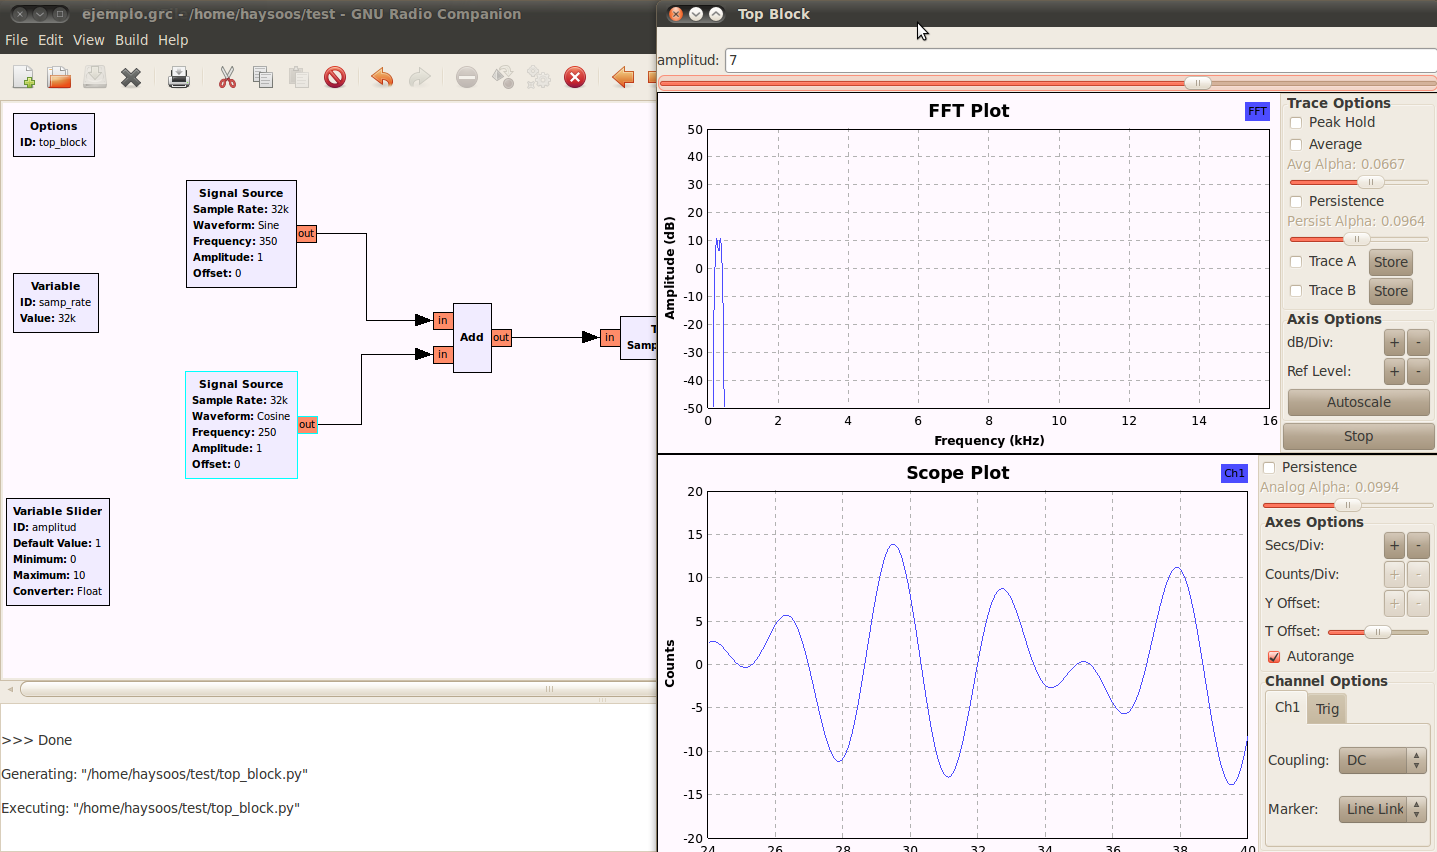
\includegraphics[width=5.5in]{figs/grc9}
  \vspace{0.1in}
  \caption{Modificaci\'on de par\'ametros por medio de bloques variables en GRC}
  \label{fig:vargrc}
\end{figure}

Todo el trabajo realizado dentro de GRC se guarda dentro de una archivo con extensi\'on \verb|.grc| y contiene la estructura del
diagrama realizado en formato XML. Una porci\'on del archivo generado por el ejemplo de este ap\'endice se muestra en el listado
\ref{ex:grc}.

\begin{lstlisting}[float, language=XML, label=ex:grc, caption={C\'odigo XML de un proyecto de GRC}]
<?xml version='1.0' encoding='ASCII'?>
<flow_graph>
  <timestamp>Sat Oct 23 11:19:29 2010</timestamp>
  <block>
    <key>variable</key>
    <param>
      <key>id</key>
      <value>samp_rate</value>
    </param>
    <param>
      <key>_enabled</key>
      <value>True</value>
    </param>
    <param>
      <key>value</key>
      <value>32000</value>
    </param>
    <param>
      <key>_coordinate</key>
      <value>(10, 170)</value>
    </param>
    <param>
      <key>_rotation</key>
      <value>0</value>
    </param>
  </block>
  .
  .
  .
  <connection>
    <source_block_id>gr_sig_source_x_0</source_block_id>
    <sink_block_id>gr_add_xx_0</sink_block_id>
    <source_key>0</source_key>
    <sink_key>0</sink_key>
  </connection>
</flow_graph>
\end{lstlisting}

Cada uno de los bloques que forman parte del grafo se definen entre las llaves \verb|<block> </block>| y dentro de estas llaves se
definen los par\'ametros del bloque en cuesti\'on. Las conexiones se definen entre las llaves \verb|<connection> </connection>|.
Cuando se ejecuta el programa, GRC traduce el archivo XML en un archivo \emph{Python} que lleva a cabo el funcionamiento del grafo
que se defini\'o. Su estructura se basa en un esqueleto pre-definido para todos los programas que genera, ya sea si son gr\'aficos o por
medio de la consola. El programa \emph{Python} generado se muestra en el listado \ref{ex:grcpython}.

\begin{lstlisting}[float=hp, breaklines=true]
#!/usr/bin/env python
##################################################
# Gnuradio Python Flow Graph
# Title: Ejemplo
# Author: Jesus Espinoza Hernandez
# Description: Suma de dos senales
# Generated: Sat Oct 23 11:19:35 2010
##################################################

from gnuradio import eng_notation
from gnuradio import gr
from gnuradio import window
from gnuradio.eng_option import eng_option
from gnuradio.gr import firdes
from gnuradio.wxgui import fftsink2
from gnuradio.wxgui import scopesink2
from grc_gnuradio import wxgui as grc_wxgui
from optparse import OptionParser
import wx

class top_block(grc_wxgui.top_block_gui):

	def __init__(self):
		grc_wxgui.top_block_gui.__init__(self, title="Ejemplo")
		_icon_path = "/usr/share/icons/hicolor/32x32/apps/gnuradio-grc.png"
		self.SetIcon(wx.Icon(_icon_path, wx.BITMAP_TYPE_ANY))

		##################################################
		# Variables
		##################################################
		self.samp_rate = samp_rate = 32000

		##################################################
		# Blocks
		##################################################
		self.gr_add_xx_0 = gr.add_vff(1)
		self.gr_sig_source_x_0 = gr.sig_source_f(samp_rate, gr.GR_COS_WAVE, 1000, 1, 0)
		self.gr_sig_source_x_1 = gr.sig_source_f(samp_rate, gr.GR_COS_WAVE, 2000, 1, 0)
		self.gr_throttle_0 = gr.throttle(gr.sizeof_float*1, samp_rate)
\end{lstlisting}

\begin{lstlisting}[float=hp, breaklines=true]
		self.wxgui_fftsink2_0 = fftsink2.fft_sink_f(
			self.GetWin(),
			baseband_freq=0,
			y_per_div=10,
			y_divs=10,
			ref_level=50,
			ref_scale=2.0,
			sample_rate=samp_rate,
			fft_size=1024,
			fft_rate=30,
			average=True,
			avg_alpha=None,
			title="Espectro",
			peak_hold=False,
		)
		self.Add(self.wxgui_fftsink2_0.win)
		self.wxgui_scopesink2_0 = scopesink2.scope_sink_f(
			self.GetWin(),
			title="Senal Original",
			sample_rate=samp_rate,
			v_scale=0,
			v_offset=0,
			t_scale=0,
			ac_couple=False,
			xy_mode=False,
			num_inputs=1,
			trig_mode=gr.gr_TRIG_MODE_AUTO,
		)
		self.Add(self.wxgui_scopesink2_0.win)

		##################################################
		# Connections
		##################################################
		self.connect((self.gr_sig_source_x_0, 0), (self.gr_add_xx_0, 0))
		self.connect((self.gr_sig_source_x_1, 0), (self.gr_add_xx_0, 1))
		self.connect((self.gr_add_xx_0, 0), (self.gr_throttle_0, 0))
		self.connect((self.gr_throttle_0, 0), (self.wxgui_scopesink2_0, 0))
		self.connect((self.gr_throttle_0, 0), (self.wxgui_fftsink2_0, 0))
\end{lstlisting}

\begin{lstlisting}[float=hp, label=ex:grcpython, caption={C\'odigo \emph{Python} generado por GRC}, breaklines=true]
	def set_samp_rate(self, samp_rate):
		self.samp_rate = samp_rate
		self.gr_sig_source_x_0.set_sampling_freq(self.samp_rate)
		self.wxgui_fftsink2_0.set_sample_rate(self.samp_rate)
		self.gr_sig_source_x_1.set_sampling_freq(self.samp_rate)
		self.wxgui_scopesink2_0.set_sample_rate(self.samp_rate)

if __name__ == '__main__':
	parser = OptionParser(option_class=eng_option, usage="%prog: [options]")
	(options, args) = parser.parse_args()
	tb = top_block()
	tb.Run(True)
\end{lstlisting}

El programa generado se puede modificar manualmente y expandirse sin utilizar GRC pero el usuario debe tener en consideraci\'on de
que si se vuelve a generar a trav\'es de GRC los cambios que se realizaron a mano se perder\'an.

El ejemplo ilustrado en este ap\'endice es un solo un fragmento de las capacidades de
\emph{GNURadio Companion}. Los bloques de los generadores de se\~nales se pueden reemplazar por
bloques que encapsulen alg\'un hardware como tarjetas de audio, el USRP o incluso tarjetas de
adquisici\'on de datos, aunque para estas es necesario crear el bloque desde cero y proporcionar los
drivers del hardware adecuados. Tambi\'en es posible trabajar con varios filtros como pasa bajas,
Hilbert y ventanas. GRC en s\'i act\'ua como una interfaz gr\'afica a los bloques de \gnuradio
facilitando as\'i su uso de una manera m\'as intuitiva. Esto permite una mejor interacci\'on con el
software para aplicaciones acad\'emicas donde la experiencia con programaci\'on no es necesaria.
